%! Author = Xandra Campo Blanco
%! Date = 6/4/25

% Preamble
\documentclass{beamer}
\usetheme[secheader]{Madrid}
\usecolortheme{dolphin}
\setbeamertemplate{navigation symbols}{}

\title[Prevención frente al acoso sexual]{Prevención y actuación temprana frente al acoso sexual y por razón de sexo, incluido en el ámbito digital}
\subtitle{Plan de formación 2025 \newline Subdirección General de RRHH e Inspección de Servicios \newline Ministerio de Ciencia, Innovación y Universidades}
\author[X. Campo]{Xandra Campo}
\institute[CIEMAT]{CIEMAT}
\date{Abril de 2025}

% Packages
\usepackage{amsmath}

\AtBeginSection{%
    \begin{frame}
        \tableofcontents[sections=\value{section}]
    \end{frame}
}

% Document
\begin{document}
    \maketitle
    \begin{frame}
        \frametitle{Prevención y actuación temprana frente al acoso sexual y por razón de sexo, incluido en el ámbito digital}
        \tableofcontents[hideallsubsections]
    \end{frame}


    \section{Sobre el curso}

    \subsection{Informacion general}
    \begin{frame}
        \frametitle{Información general}
        \textbf{Organización}:
        \begin{description}[Other description]
            \item[Organizador] Subdirección General de RRHH e Inspección de Servicios del MICIU
            \item[Destinatarios] Personal del MICIU y organismos dependientes
            \item[Plan de formación] 2025
            \item[Área formativa] Igualdad de Género
            \item[Duración] 9 horas
        \end{description}
        \textbf{Profesorado}:
        \begin{description}[Other description]
            \item[Mar Liñán] Responsable del Servicio de PRL del MICIU
            \item[Ignacio Cudeiro] Inspector General de Servicios del MICIU
            \item[Paz Lloria] Catedrática de Derecho penal, Universitat de València
        \end{description}
    \end{frame}

    \subsection{Antecedentes y motivación}
    \begin{frame}
        \frametitle{Antecedentes y motivación}
        \textbf{Leyes relevantes}:
        \begin{itemize}
            \item \textit{Ley Orgánica 3/2007}: Igualdad efectiva de hombres y mujeres
            \item \textit{Ley Orgánica 10/2022}: Garantía integral de la libertad sexual
            \item \textit{Ley 17/2022}: Modificación de la Ley 14/2011 de Ciencia, Tecnología e Innovación
        \end{itemize}
        \textbf{Requerimientos}:
        \begin{itemize}
            \item Informar, sensibilizar y formar al personal sobre acoso y violencia de género, incluyendo el ámbito digital y la I+D+I
            \item Planes de Igualdad de Género y Protocolos contra el acoso con seguimiento anual para agentes públicos del Sistema Español de Ciencia, Tecnología e Innovación (SECTI)
        \end{itemize}
    \end{frame}

    \begin{frame}
        \frametitle{Antecedentes y motivación}
        \textbf{Compromiso del ministerio}:
        \begin{itemize}
            \item Erradicar el acoso sexual y por razón de sexo en instituciones, universidades y centros de investigación
            \item Promover entornos laborales diversos, inclusivos, seguros e igualitarios
            \item Garantizar formación adecuada para la prevención, detección temprana y abordaje de situaciones de acoso
        \end{itemize}
        \textbf{Contexto actual}:
        \begin{itemize}
            \item Persistencia del acoso sexual y por razón de sexo en entornos laborales jerarquizados
            \item Revolución de las TIC, que ha exacerbado las desigualdades de género y la violencia contra las mujeres, incluyendo el ámbito de la I+D+I
        \end{itemize}
    \end{frame}

    \subsection{Objetivos y destinatarios}
    \begin{frame}
        \frametitle{Objetivos y destinatarios}
        \textbf{Objetivos}:
        \begin{itemize}
            \item Proporcionar formación adecuada para la prevención, detección y abordaje del acoso sexual y por razón de sexo en el ámbito laboral, incluyendo entornos digitales
            \item Destacar los desequilibrios de poder en espacios digitales y presentar la normativa existente y recomendaciones prácticas para prevenir y erradicar estas situaciones
        \end{itemize}
        \textbf{Destinatarios}:
        \begin{itemize}
            \item Todo el personal del Ministerio de Ciencia, Innovación y Universidades (MICIU) y sus organismos dependientes
            \item Especialmente dirigido a personal de RRHH, comités de igualdad, comités de selección, programas de evaluación, investigadores/as principales, y personal pre-directivo y directivo
        \end{itemize}
    \end{frame}


    \section{Normativa}

    \subsection{Normativa internacional y europea}
    \begin{frame}{Normativa internacional y europea}
        \textbf{Normativa internacional}
        \begin{itemize}
            \item \textit{Convenio 190} y \textit{Recomendación 206} (OIT, 2019): Eliminación de la violencia y el acoso en el mundo del trabajo
        \end{itemize}
        \textbf{Normativa europea}
        \begin{itemize}
            \item \textit{Directiva 2006/54/CE}: Igualdad de trato entre hombres y mujeres en materia de empleo y ocupación
            \item \textit{Directiva 2019/1158}: Conciliación de la vida familiar y profesional
            \item \textit{Directiva 2024/1385}: Lucha contra la violencia contra las mujeres y la violencia doméstica
            \item \textit{Convenio de Estambul} (2011): Prevención y lucha contra la violencia contra las mujeres y la violencia doméstica
            \item \textit{Carta de los Derechos Fundamentales de la UE} (2009): Art. 21 y 23
        \end{itemize}
    \end{frame}

    \subsection{Normativa española}
    \begin{frame}{Normativa española}
        \textbf{Ámbito general}
        \begin{itemize}
            \item \textit{Constitución Española}: Art. 9.2, 10.1, 14, 15, 18.1, 35.1
            \item \textit{Ley 31/1995}: Prevención de Riesgos Laborales
        \end{itemize}
        \textbf{Ámbito disciplinario}
        \begin{itemize}
            \item \textit{RD 33/1986}: Régimen disciplinario de los funcionarios de la AGE
            \item \textit{RD 799/2005}: Inspecciones generales de servicios de los departamentos ministeriales
            \item \textit{RDL 2/2015}: Estatuto de los Trabajadores
            \item \textit{RDL 5/2015}: Ley del Estatuto Básico del Empleado Público
        \end{itemize}
        \textbf{Ámbito penal}
        \begin{itemize}
            \item \textit{RD de 14 de septiembre de 1882}: Ley de enjuiciamiento criminal
            \item \textit{LO 10/1995}: Código Penal, art. 184
            \item \textit{Ley 4/2016}: Estatuto de la víctima del delito
        \end{itemize}
    \end{frame}

    \begin{frame}{Normativa española}
        \textbf{Ámbito igualdad de genero}
        \begin{itemize}
            \item \textit{LO 1/2004}: Protección integral contra la violencia de género
            \item \textit{LO 3/2007}: Igualdad Efectiva de Mujeres y Hombres
            \item \textit{Res. SE FP julio 2011}: Protocolo de actuación frente al AS y ARS en la AGE
            \item \textit{RD 901/2020}: Regulación de los planes de igualdad y su registro
            \item \textit{RD 902/2020}: Igualdad retributiva entre mujeres y hombres
            \item \textit{Res. SE FP diciembre 2020}: III Plan de igualdad de género en la AGE
            \item \textit{LO 8/2021}: Protección integral de la infancia frente a la violencia
            \item \textit{LO 10/2022}: Garantía integral de la libertad sexual
            \item \textit{Ley 15/2022}: Igualdad de trato y la no discriminación
            \item \textit{RD 247/2024}: Protocolo de actuación frente al AS y ARS en la AGE
        \end{itemize}
    \end{frame}


    \section{Definiciones}

    \subsection{Necesidad de definir}
    \begin{frame}{Definiciones: Necesidad}
        \textbf{Necesidad de definir}
        \begin{itemize}
            \item Definir conceptos, conductas, causas y efectos del acoso sexual y por razón de sexo es esencial para su comprensión y prevención, y para asegurar la seguridad jurídica y la presunción de inocencia
        \end{itemize}
        El acoso sexual y por razón de sexo está:
        \begin{itemize}
            \item \textbf{Prohibido} por Ley 3/2007, Igualdad efectiva entre mujeres y hombres
            \item Considerado \textbf{infracción muy grave} por el Estatuto de los Trabajadores, Estatuto Básico del Empleado Público, Ley de infracciones y sanciones del orden social
            \item Tipificado como \textbf{delito} en el Código Penal (Art. 184)
        \end{itemize}
    \end{frame}

    \subsection{Acoso sexual}
    \begin{frame}{Definiciones: Acoso sexual}
        Ley Orgánica 3/2007, Igualdad efectiva de mujeres y hombres, art. 7
        \begin{itemize}
            \item \textbf{Definición}: Comportamiento verbal o físico de naturaleza sexual, con el propósito o
            efecto de atentar contra la dignidad de una persona, en particular cuando se crea un entorno
            intimidatorio, degradante u ofensivo, con independencia de la jerarquía sobre la víctima
            \item \textbf{Chantaje sexual}: Se produce cuando la persona acosadora ocupa un puesto jerárquicamente
            superior o cuando sus decisiones pueden tener efectos sobre el empleo o las condiciones de trabajo de la
            víctima
            \item \textbf{Acoso ambiental}: Comportamiento que produce un entorno intimidatorio, degradante u ofensivo
            para la persona que lo sufre
        \end{itemize}
    \end{frame}

    \begin{frame}{Definiciones: Acoso sexual}
        Código Penal, Delitos contra la libertad e indemnidad sexuales, art.184
        \small
        \begin{itemize}
            \item El que \textbf{solicite favores de naturaleza sexual}, para sí o para un tercero, en el ámbito de una relación
            laboral, docente o de prestación de servicios, continuada o habitual, provocando a la
            víctima una situación objetiva y gravemente intimidatoria, hostil o humillante, será castigado con pena de
            prisión de 3 a 5 meses o multa de 6 a 10 meses
            \item Si el culpable comete el hecho prevaliéndose de una \textbf{situación de superioridad}
            laboral, docente o jerárquica, o con el anuncio expreso o tácito de causar a la víctima un mal relacionado con
            las legítimas expectativas que pueda tener en el ámbito de la indicada relación, la pena será de prisión
            de 5 a 7 meses o multa de 10 a 14 meses
            \item Cuando la víctima sea \textbf{especialmente vulnerable}, por razón de su edad, enfermedad o situación, la pena
            será de prisión de 5 a 7 meses o multa de 10 a 14 meses (apartado 1) y
            de prisión de 6 meses a 1 año (apartado 2)
        \end{itemize}
    \end{frame}

    \subsection{Acoso por razón de sexo}
    \begin{frame}{Definiciones: Acoso por razón de sexo}
        Ley Orgánica 3/2007, Igualdad efectiva de mujeres y hombres, art. 7
        \begin{itemize}
            \item Cualquier \textbf{comportamiento realizado en función del sexo de una persona}, con el propósito o el efecto de
            atentar contra su dignidad, y de crea un entorno intimidatorio, degradante u ofensivo, con independencia de
            la jerarquía o inexistencia de jerarquía de la persona que la realiza sobre la víctima
            \item Incluye todo trato desfavorable relacionado con el embarazo, la maternidad, paternidad o asunción de
            otros cuidados familiares, así como trato desfavorable en función de la identidad y/o expresión de género u
            orientación sexual
        \end{itemize}
    \end{frame}

    \subsection{Delitos relacionados}
    \begin{frame}{Definiciones: Delitos relacionados}
        Código Penal, De las coacciones, art. 173
        \small
        \begin{itemize}
            \item El que infligiera a otra persona un trato degradante, menoscabando gravemente su \textbf{integridad moral}, será castigado con
            pena de prisión de 6 meses a 2 años
            \item Será castigado con la misma pena el que, en el ámbito de cualquier \textbf{relación laboral} o funcionarial y prevaliéndose de
            su relación de superioridad, realicen contra otro de forma reiterada actos hostiles o humillantes que, sin llegar a constituir
            trato degradante, supongan grave acoso contra la víctima
            \item Quien cause injuria o vejación injusta de carácter leve, cuando la victima encaje en el \textbf{ap. 2 del art. 173},
            será castigado con pena de localización permanente o trabajos en beneficio de la comunidad de 5 a 30 días,
            o multa de 1 a 4 meses en los supuestos del ap. 2 del art. 84
            \item Las mismas penas se impondrán a quienes se dirijan a otra persona con expresiones, comportamientos o proposiciones
            \textbf{de carácter sexual} que creen a la víctima una situación objetivamente humillante, hostil o intimidatoria, sin llegar a
            constituir otros delitos de mayor gravedad
        \end{itemize}
    \end{frame}


    \section{AS y ARS como riesgo psicosocial en el ámbito laboral}

    \subsection{Visión del AS y ARS desde la perspectiva de la PRL}
    \begin{frame}{Visión del AS y ARS desde la perspectiva de la PRL}
        \textbf{Definiciones}:
        \begin{itemize}
            \item \textbf{Riesgo laboral}: posibilidad de que un trabajador sufra un daño derivado del trabajo, valorando su probabilidad severidad
            \item \textbf{Factores de riesgo psicosocial}: Condiciones de trabajo deficientes que aumentan la probabilidad de consecuencias negativas para la seguridad y salud de los trabajadores
            \begin{itemize}
                \item \textit{Contenido de trabajo}: Fragmentación, complejidad, repetitividad,
                \item \textit{Carga de trabajo}: Infracarga, sobrecarga, ritmo alto, interrupciones
                \item \textit{Tiempo de trabajo}: Nocturnidad, turnicidad, jornadas largas
                \item \textit{Participación}: Falta de autonomía, déficit de iniciativa y liderazgo
                \item \textit{Desempeño de rol}: Indefinición, conflicto de valores, sobrecarga
                \item \textit{Desarrollo profesional}: Estancamiento, contratos precarias
                \item \textit{Relaciones interpersonales}: Escaso apoyo social, conflictos
                \item \textit{Equipos de trabajo}: Tecnologías, herramientas, entorno físico
            \end{itemize}
        \end{itemize}
    \end{frame}

    \begin{frame}{Visión del AS y ARS desde la perspectiva de la PRL}
        \begin{itemize}
            \item \textbf{Principios de la actividad preventiva}:
            \begin{itemize}
                \item Evitar y evaluar riesgos y combatirlos en su origen
                \item Adaptar el trabajo a la persona y tener en cuenta la evolución técnica
                \item Sustituir lo peligroso por lo seguro
                \item Planificar la prevención (técnica, organización y condiciones de trabajo)
                \item Priorizar la protección colectiva sobre la individual
                \item Instruir adecuadamente a los trabajadores
            \end{itemize}
            \item \textbf{Proceso de mejora continua}:
            \begin{itemize}
                \item Identificación y evaluación
                \item Planificación de la actividad preventiva
                \item Intervención psicosocial
                \item Evaluación seguimiento y control
            \end{itemize}
        \end{itemize}
    \end{frame}

    \begin{frame}{Visión del AS y ARS desde la perspectiva de la PRL}
        \begin{itemize}
            \item \textbf{Herramientas para evaluar los riesgos psicosociales}:
            \begin{itemize}
                \item \textit{Encuesta de clima laboral}: Cultura organizacional y el ambiente
                \item \textit{Evaluación de riesgos psicosociales}: Identificación y prevención de factores de riesgo que afectan la salud mental
            \end{itemize}
            \item \textbf{Metodologías de obtención de información}:
            \begin{itemize}
                \item \textit{Cuantitativas}: Cantidad de fenómenos (cuestionarios)
                \item \textit{Cualitativas}: Descripción de fenómenos (entrevistas, grupos de discusión)
            \end{itemize}
        \end{itemize}
    \end{frame}

    \subsection{Percepción social del acoso sexual y por razón de sexo}
    \begin{frame}{Encuesta de percepción social del AS y ARS}
        \begin{columns}
            \column{0.4\textwidth}
            \begin{itemize}
                \item \textbf{Objetivo}: Recoger las percepciones sobre la violencia sexual y su nivel de aceptación en la sociedad
                \item \textbf{Innovación}: 1ª encuesta sólo de violencia sexual
                \item \textbf{Autor}: CIS y Del. Gob. Violencia de Género
                \item \textbf{Muestra}: 2.465 personas, mas de 16 años, España
            \end{itemize}
            \column{0.6\textwidth}
            \begin{figure}
                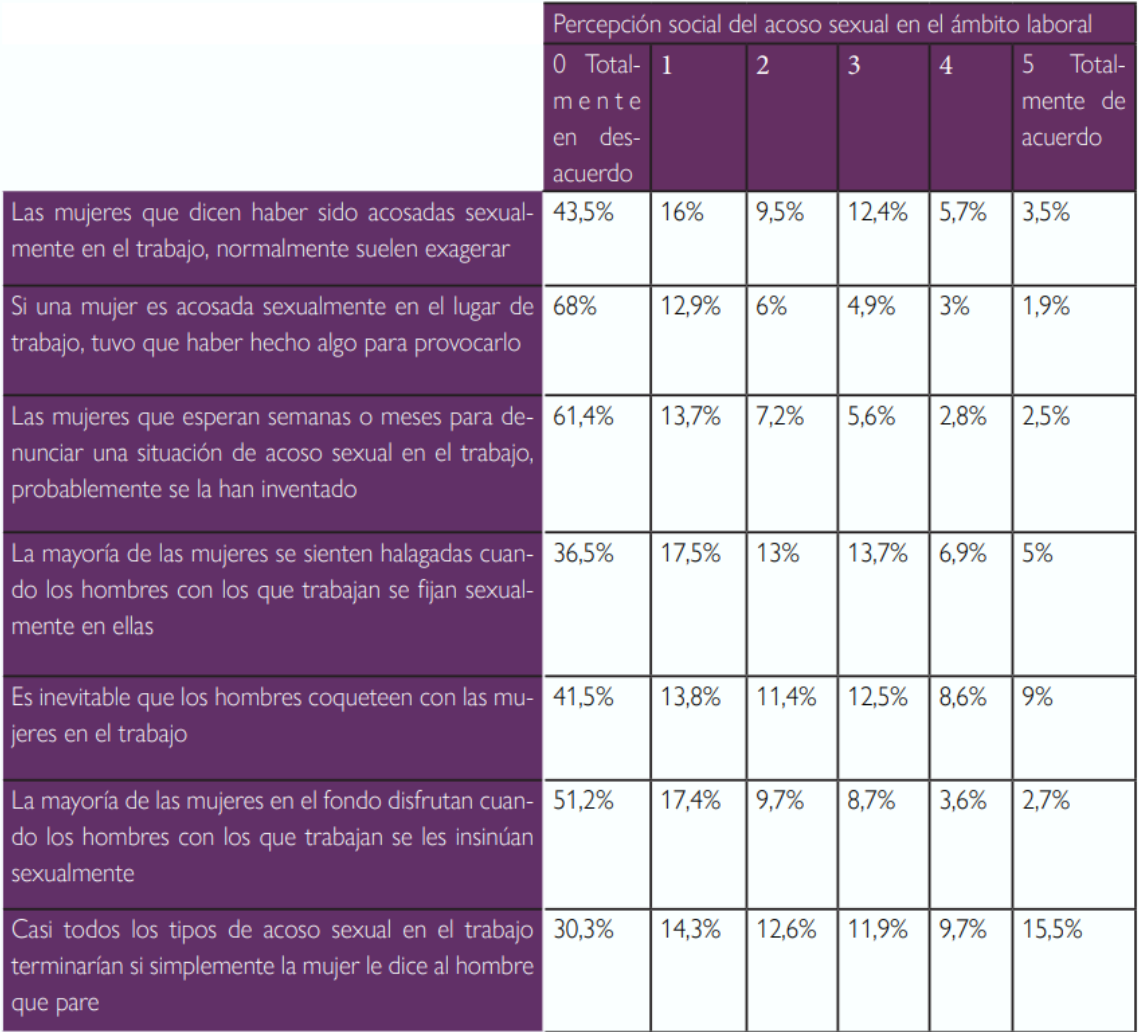
\includegraphics[width=\textwidth]{assets/encuesta_percepcion_social}
            \end{figure}
        \end{columns}
    \end{frame}

    \subsection{Perfil de víctima y acosador/a}
    \begin{frame}{Perfil de víctima y acosador/a}
        \textbf{Perfil de la víctima}: Mayoritariamente mujeres, especialmente aquellas en situaciones vulnerables
        \begin{itemize}
            \item Solas con responsabilidades familiares
            \item Sectores laborales masculinizados y/o precarios
            \item Jóvenes en su primer trabajo
            \item Discapacidad
            \item Migrantes o de minorías étnicas
        \end{itemize}
        \textbf{Perfil del acosador}: Mayoritariamente varones
        \begin{itemize}
            \item Superiores jerárquicos, compañeros o clientes
            \item Cualquier estrato social, nivel ocupacional y categoría profesional
            \item No hay un rango de edad específico
            \item Creencias y actitudes sexistas vinculadas a la masculinidad tradicional
        \end{itemize}
    \end{frame}

    \subsection{Consecuencias del acoso sexual y por razón de sexo}
    \begin{frame}{Consecuencias del acoso sexual y por razón de sexo}
        \begin{itemize}
            \item \textbf{Ámbito físico y fisiológico}: Enfermedades coronarias, trastornos dermatológicos, endocrinos, gastrointestinales, respiratorios, musculoesqueléticos, inmunológicos
            \item \textbf{Ámbito cognitivo}: Déficit de atención, dificultades de concentración, déficit de memoria, pensamientos recurrentes
            \item \textbf{Ámbito emocional}: Irritabilidad, ansiedad, temor, impulsividad, desconfianza, depresión
            \item \textbf{Ámbito conductual}: Sedentarismo, abuso de sustancias, conductas peligrosas, absentismo, suicidio
            \item \textbf{Ámbito social}: Aislamiento, conflictos, ausencia de comunicación
            \item \textbf{Ámbito organizacional}: Mayor absentismo, menor productividad, estancamiento laboral, despidos, responsabilidad legal
        \end{itemize}
    \end{frame}

    \begin{frame}{Consecuencias del acoso sexual y por razón de sexo}
        \begin{itemize}
            \item En materia laboral, el \textbf{acoso sexual} es considerado como \textbf{riesgo laboral}, del cual pueden derivarse lesiones corporales, ya sean de orden físico o psíquico
            \item Sin embargo, mayoritariamente se consideran las \textbf{consecuencias del AS y ARS} como \textbf{contingencia común}, no como accidente de trabajo
            \item \textbf{Requisitos} para que sean considerados \textbf{accidente laboral}: existencia y acreditación de la conducta acosadora y del daño en la víctima, identificación de un nexo causal que vincule la lesión con el trabajo
            \item \textbf{Determinación de contingencias}: de oficio por el INSS, a instancias de la persona, su representante legal o las mutuas de accidentes de trabajo y enfermedades profesionales de la SS.
        \end{itemize}
    \end{frame}

    \subsection{Asistencia/apoyo a las víctimas de acoso}
    \begin{frame}{Asistencia/apoyo a las víctimas de acoso}
        \textbf{¿Qué puedo hacer si me siento acosada/o?}
        \begin{itemize}
            \item \textit{Solicitar información}: Empresa, representación legal de los trabajadores, servicio de información del Instituto de la Mujer
            \item \textit{Resolución informal del conflicto}: Conforme al protocolo de la empresa (confidencialidad)
            \item \textit{Presentar una denuncia}: Inspección de Trabajo y Seguridad Social, Policía o juzgado de guardia (no anónimas)
        \end{itemize}
        \textbf{¿En qué consiste la asistencia y apoyo a las víctimas?}
        \begin{itemize}
            \item Información sobre procedimientos, derechos, medidas disciplinarias y penales
            \item Asistencia psicológica y médica, apoyo emocional y acompañamiento
            \item Asesoramiento jurídico y profesional
            \item Ejecución de medidas y prevención de represalias
        \end{itemize}
    \end{frame}

    \subsection{Detección temprana del acoso sexual y por razón de sexo}
    \begin{frame}{Detección temprana del acoso sexual y por razón de sexo}
        \begin{itemize}
            \item \textbf{Estrategias de detección}: basadas en la observacion, comunicación y formación
            \item \textbf{Observación}: Señales de alerta: cambios en el comportamiento de la víctima, conductas inadecuadas en el ambiente de trabajo, indicios en la comunicación digital
            \item \textbf{Comunicación}: Canales de comunicación seguros, supervisión y liderazgo activo, protocolos de intervención rápida
            \item \textbf{Formación}: Formación y sensibilización, encuestas y evaluaciones internas
            \item \textbf{Papel de los testigos}: Observar cambios en la actitud de la víctima o del agresor, alertar de comportamientos inapropiados, apoyar a la persona afectada
        \end{itemize}
    \end{frame}

    \subsection{Prevención del acoso sexual y por razón de sexo}
    \begin{frame}{Prevención del acoso sexual y por razón de sexo}
        \framesubtitle{Por parte de las personas trabajadoras}
        \begin{itemize}
            \item \textbf{Derechos}: derecho a un entorno de trabajo saludable, a no sufrir acoso, a informar de posibles situaciones de acoso sin sufrir represalias
            \item \textbf{Obligaciones}: Tratar a los demás con respecto y cooperar con la empresa en la investigación de una denuncia interna de acoso
            \item \textbf{Recomendaciones}:
            \begin{itemize}
                \item Potenciar un papel activo en la garantía de la tolerancia 0 ante el acoso
                \item Mantener conducta propia y hacia los demás que no sean ofensivos
                \item Dejando claro que encuentran ciertos comportamientos inaceptables
                \item Dar soporte a las personas que puedan sufrir acoso
            \end{itemize}
        \end{itemize}
    \end{frame}
    \begin{frame}{Prevención del acoso sexual y por razón de sexo}
        \framesubtitle{Por parte de las empresas}
        \textbf{Obligaciones}
        \begin{itemize}
            \item Adquisición de un compromiso firme de tolerancia 0 ante el acoso.
            \item Creación de un marco de relaciones laborales igualitarias.
        \end{itemize}
        Medios
        \begin{itemize}
            \item \textbf{Compromiso de la empresa}: Formalizar el compromiso en documentos corporativos, generar confianza y fomentar la colaboración
            \item \textbf{Políticas de igualdad}: Estilos de gestión y organización del trabajo que dificulten el acoso, medidas específicas para garantizar la plena integración e igualdad efectiva de las mujeres
            \item \textbf{Respuesta de la organización}: Compromiso explícito contra el acoso, desaprobación de conductas ofensivas, aplicación de medidas disciplinarias severas
        \end{itemize}
    \end{frame}

    \begin{frame}{Recursos disponibles en el MICIU}
        \begin{itemize}
            \item \textbf{Protocolos de actuación}: frente al acoso laboral, al AS y ARS, frente a la discriminación por orientacion o identidad sexual, expresion de genero y caracacteristicas sexuales
            \item Listado de personas habilitadas para \textbf{asesoría confidencial} y \textbf{unidad de activación} frente al acoso
            \item \textbf{Material audiovisual}: Identificar y erradicar comportamientos micromachistas, tolerancia cero frente al AS y ARS
            \item \textbf{Cursos específicos}: Plan de formación en igualdad y prevención de riesgos laborales
        \end{itemize}
    \end{frame}


    \section{Protocolo frente al acoso sexual y acoso por razón de sexo}

    \subsection{Marco de actuación}
    \begin{frame}{Marco de actuación}
        \begin{itemize}
            \item Ámbito administrativo: medidas organizativas
            \item Ámbito administrativo: medidas disciplinarias
            \item Ámbito penal
        \end{itemize}
    \end{frame}

    \subsection{Ámbito administrativo: Medidas organizativas}
    \begin{frame}{Ámbito administrativo: Medidas organizativas}
        \begin{itemize}
            \item Garantías y protección
            \item Prevención de riesgos
            \item Formación
            \item Coordinación
            \item Comunicación, consulta y denuncia
            \item Recomendaciones de actuación
            \item Protocolos y otras instrucciones de actuación (transversal)
        \end{itemize}
    \end{frame}

    \begin{frame}{Ámbito administrativo: Medidas organizativas}
        \textbf{Garantías y protección}
        \begin{itemize}
            \item Asegurar el respeto y la \textbf{protección} de todas las personas implicadas
            \item Garantizar la \textbf{confidencialidad} y el respeto a la intimidad y la dignidad
            \item Actuar con rapidez y diligencia, asegurando seguridad y coordinación
            \item Mantener la \textbf{imparcialidad} en todas las etapas del proceso
            \item Proporcionar \textbf{información} sobre el protocolo, asistencia y posibles vías disciplinarias y penales
            \item Prohibir \textbf{represalias} contra quienes denuncien o participen en el proceso
            \item Implementar \textbf{medidas provisionales} durante los procedimientos disciplinarios o penales
            \item Considerar la \textbf{interseccionalidad} con otras garantías de derechos
        \end{itemize}
    \end{frame}

    \begin{frame}{Ámbito administrativo: Medidas organizativas}
        \textbf{Prevención de riesgos}
        \begin{itemize}
            \item Realizar un análisis de \textbf{riesgos} en el entorno laboral: encuestas, comunicaciones y estudios
            \item Identificar y evaluar los \textbf{factores de riesgo} y establecer medidas preventivas
            \item Implementar \textbf{medidas de organización} de personal, del trabajo y de las instalaciones: procedimientos, guías, manuales, codigos eticos
        \end{itemize}
        \textbf{Formación}
        \begin{itemize}
            \item Sobre igualdad de trato y oportunidades entre mujeres y hombres, prevención de la violencia de género
            \item Formacion general, capacitacion especifica, campañas de prevencion y concienciación
        \end{itemize}
    \end{frame}

    \begin{frame}{Ámbito administrativo: Medidas organizativas}
        \textbf{Coordinación}
        \begin{itemize}
            \item Unidades de información y tratamiento:
            \begin{itemize}
                \item Unidades de recepción de denuncias
                \item Asesoría confidencial
            \end{itemize}
            \item Titulares de los órganos superiores y personal directivo:
            \begin{itemize}
                \item \textbf{Coordinación} con estas unidades, primera línea de detección temprana y prevención
                \item \textbf{Velar} por un trato respetuoso y digno, vigilancia preventiva, fomentar un clima laboral libre de conductas discriminatorias
                \item \textbf{Aplicar} medidas organizativas preventivas o destinadas a poner fin a las situaciones detectadas, así como medidas provisionales o cautelares derivadas de procedimientos disciplinarios o jurisdiccionales
            \end{itemize}
        \end{itemize}
    \end{frame}

    \begin{frame}{Ámbito administrativo: Medidas organizativas}
        \textbf{Comunicación, consulta y denuncia}
        \begin{itemize}
            \item \textbf{Activación del protocolo}
            \begin{itemize}
                \item Puede ser verbal o escrita, incluyendo un modelo de comunicación en el anexo, por correo electrónico (\href{mailto:acoso@ciencia.gob.es}{acoso@ciencia.gob.es}) o verbalmente ante la Unidad de activación
                \item Puede ser solicitada por la víctima, su representante legal, la representación de empleados públicos, o cualquier persona con conocimiento de hechos constitutivos de acoso
            \end{itemize}
            \item \textbf{Denuncia}
            \begin{itemize}
                \item Debe \textbf{contener} un relato claro de los hechos, identidad del presunto infractor y de la víctima, y datos identificativos del denunciante
                \item Se favorece la \textbf{confidencialidad} mediante la anonimización de datos personales en los documentos de tramitación
                \item Puede ser \textbf{anónima} según la Ley 2/2023, pero no para la vía penal y disciplinaria
            \end{itemize}
        \end{itemize}
    \end{frame}

    \begin{frame}{Ámbito administrativo: Medidas organizativas}
        \textbf{Recomendaciones de actuación}
        \begin{itemize}
            \item El \textbf{protocolo concluye} con un informe que incluye recomendaciones de actuación
            \item El \textbf{informe} puede recomendar iniciar un procedimiento disciplinario si hay indicios de falta
            \item Si se aprecian \textbf{indicios de delito}, se trasladará al Ministerio Fiscal para la vía penal
            \item Otras recomendaciones pueden incluir \textbf{medidas organizativas} para interrumpir o prevenir situaciones detectadas
            \item \textbf{Medidas organizativas} pueden ser: traslado de puesto de la víctima o del agresor, y suspensión de funciones por un máximo de seis meses
        \end{itemize}
    \end{frame}

    \begin{frame}{Ámbito Administrativo: Medidas Organizativas}
        \textbf{Real Decreto 247/2024, Protocolo de actuación en la AGE, art. 62}

        Principios rectores:
        \begin{itemize}
            \item \textbf{Compromiso} de la AGE de prevenir y no tolerar el acoso sexual y el acoso por razón de sexo
            \item \textbf{Instrucción} a todo el personal de su deber de respetar la dignidad de las personas y su derecho a la intimidad, así como la igualdad de trato entre mujeres y hombres
            \item \textbf{Tratamiento reservado} de las denuncias de hechos que pudieran ser constitutivos de acoso sexual o de acoso por razón de sexo, sin perjuicio de lo establecido en la normativa de régimen disciplinario
            \item \textbf{Identificación} de las personas responsables de atender a quienes formulen una queja o denuncia
        \end{itemize}
    \end{frame}

    \subsection{Ámbito administrativo: Medidas discilpinarias}
    \begin{frame}{Ámbito Administrativo: Medidas discilpinarias}
        \begin{itemize}
            \item \textbf{Régimen disciplinario} (Art. 93.1 y 94.1 TREBEP)
            \begin{itemize}
                \item Sujetos: Funcionarios públicos y personal laboral
                \item Corrección disciplinaria de las infracciones por parte de las Administraciones Publicas
            \end{itemize}
            \item \textbf{Principios rectores} (Art. 94.2 TREBEP)
            \begin{itemize}
                \item Principio de legalidad y tipicidad de las faltas y sanciones
                \item Principio de irretroactividad de las disposiciones sancionadoras no favorables y de retroactividad de las favorables al presunto infractor
                \item Principio de proporcionalidad de la sanción respecto a la falta
                \item Principio de culpabilidad
                \item Principio de presunción de inocencia
            \end{itemize}
            \item \textbf{Competencia para incoar} expediente disciplinario
            \begin{itemize}
                \item Subsecretario: Faltas graves y muy graves
                \item Director/Presidente: Faltas leves en su ámbito
                \item Subsecretario: Faltas leves en servicios centrales
            \end{itemize}
        \end{itemize}
    \end{frame}

    \begin{frame}{Ámbito Administrativo: Medidas discilpinarias}
        \begin{itemize}
            \item \textbf{Graduación de las faltas} (Art. 95.3 TREBEP)
            \begin{itemize}
                \item Grado de vulneración de la legalidad.
                \item Gravedad de los daños al interés público.
                \item Descrédito para la imagen pública de la Administración.
            \end{itemize}
            \item \textbf{Faltas muy graves} (Art. 95.b TREBEP)
            \begin{itemize}
                \item Discriminación o acoso por origen racial, religión, discapacidad, edad, sexo, orientación sexual, etc
            \end{itemize}
            \item \textbf{Faltas Graves} (Art. 7.1 RD33/1986)
            \begin{itemize}
                \item Abuso de autoridad en el ejercicio del cargo
                \item Grave desconsideración con superiores, compañeros o subordinados
                \item Atentado grave a la dignidad de funcionarios o de la Administración
                \item Grave falta de consideración con los administrados
            \end{itemize}
        \end{itemize}
    \end{frame}

    \begin{frame}{Ámbito Administrativo: Medidas discilpinarias}
        \begin{itemize}
            \item \textbf{Terminación del procedimiento}
            \begin{itemize}
                \item Archivo de actuaciones
                \item Suspensión del procedimiento y remisión a la Fiscalía
                \item Imposición de sanción
            \end{itemize}
            \item \textbf{Sanciones y medidas cautelares}
            \begin{itemize}
                \item Separación del servicio o despido disciplinario
                \item Suspensión firme de funciones o de empleo y sueldo
                \item Traslado forzoso, demérito o apercibimiento
            \end{itemize}
            \item \textbf{Prolongación de medidas}
            \begin{itemize}
                \item Cese de medidas cautelares tras la sanción
                \item Posibilidad de mantener la situación de traslado
                \item Necesidad de reformas normativas para mantener medidas que afectan a derechos
            \end{itemize}
        \end{itemize}
    \end{frame}

    \subsection{Medidas administrativas en el MICIU}
    \begin{frame}{Protocolo de actuación del MICIU}
        \begin{itemize}
            \item \textbf{Aprobación}: La Subsecretaría de Ciencia, Innovación y Universidades adapta el protocolo de actuación frente al acoso sexual y por razón de sexo de la AGE
            \item \textbf{Cobertura}: Incluye todas las formas de acoso, incluyendo ciberacoso, y aplica a colaboradores sin relación laboral
            \item \textbf{Declaración institucional}: Rechazo rotundo a todo tipo de acoso sexual y por razón de sexo
            \item \textbf{Contenido}:
            \begin{itemize}
                \item Definiciones, obligaciones y prohibiciones
                \item Directivos con personal a cargo
                \item Medidas y canales de consulta y denuncia
                \item Unidad de activación, Asesoría Confidencial, y Comité de Asesoramiento
            \end{itemize}
        \end{itemize}
    \end{frame}

    \begin{frame}{Protocolo de actuación del MICIU}
        \textbf{Asesoría Confidencial}
        \begin{itemize}
            \item Asistir y asesorar a la víctima, informando sobre derechos y actuaciones
            \item Elaboración de informes técnicos
            \item Estudio de los hechos y entrevistar a los implicados
            \item Comunicación a la Unidad de activación frente al acoso si hay indicios suficientes de acoso
        \end{itemize}
        \textbf{Comité de Asesoramiento}
        \begin{itemize}
            \item Miembros designados por la Subsecretaría
            \item Incluye expertos en igualdad y representantes del personal
            \item Incluye representantes del Departamento y del Ministerio
            \item Los miembros no pueden intervenir en las etapas previas o posteriores a la constitución del comité
        \end{itemize}
    \end{frame}

    \begin{frame}{Protocolo de actuación del MICIU}
        \textbf{Proceso de activación}
        \begin{itemize}
            \item Comunicación a la unidad receptora
            \item Asignación a Asesoría Confidencial (24 horas)
            \item Asesoría Confidencial: Investigación, conclusiones e informe de valoración (10 días)
            \item Alegaciones de la víctima (10 días)
            \item Constitución del Comité de Asesoramiento (7 días)
            \item Comité de Asesoramiento: Investigación, conclusiones e informe final (20 días)
        \end{itemize}
        \textbf{Informe final con recomendaciones}
        \begin{itemize}
            \item Adopción de medidas organizativas que permitan la protección de la víctima y la prevención y cese del acoso
            \item Iniciar la vía disciplinaria o el traslado a la vía jurisdiccional penal
        \end{itemize}
    \end{frame}

    \subsection{Ámbito penal}
    \begin{frame}{Regimen en el ámbito penal}
        \begin{itemize}
            \item \textbf{Art. 191 Código Penal}
            \begin{itemize}
                \item Denuncia necesaria para proceder por delitos de agresiones, acoso o abusos sexuales
                \item Denuncia puede ser presentada por la víctima, su representante legal o el Ministerio Fiscal
                \item El perdón del ofendido no extingue la acción penal ni la responsabilidad
            \end{itemize}
            \item \textbf{Art. 262 LECrim}
            \begin{itemize}
                \item Los que por razón de sus cargos, profesiones u oficios tuvieren noticia de algún delito público, estarán obligados a denunciarlo inmediatamente
            \end{itemize}
            \item \textbf{Art. 94.3 TREBEP}
            \begin{itemize}
                \item Suspensión del procedimiento disciplinario si hay indicios de criminalidad, informando al Ministerio Fiscal.
                \item Hechos probados por resoluciones judiciales firmes vinculan a la Administración.
            \end{itemize}
        \end{itemize}
    \end{frame}

    \begin{frame}{Penas en el ámbito penal y su efecto administrativo}
        \begin{itemize}
            \item \textbf{Penas cautelares previas} o durante el procedimiento penal: Prohibición de aproximación o de residencia
            \item \textbf{Penas} impuestas por el juez una ves se ha dictado sentencia: Privativas de libertad o inhabilitación
            \item \textbf{Penas que se prolongan} trans el fin del procedimiento judicial: Prohibición de aproximación o de residencia
        \end{itemize}
    \end{frame}

    \begin{frame}{Unidades especializadas en el ámbito penal}
        \begin{itemize}
            \item Fiscalía de Sala de Violencia sobre la Mujer y secciones en Fiscalías Provinciales
            \item Unidad de Coordinación de Violencia sobre la Mujer de la Fiscalía General del Estado
            \item Observatorio de Violencia Doméstica y de Género del Consejo General del Poder Judicial
            \item Delegación del Gobierno contra la Violencia de Género
            \item Teléfono gratuito 016
        \end{itemize}
    \end{frame}


    \section{Acoso y violencia de género en el ámbito digital}

    \subsection{La sociedad digital}
    \begin{frame}{La sociedad digital}
        \begin{itemize}
            \item La digitalización ha transformado profundamente la interacción social, facilitando tanto la comunicación como la comisión de delitos
            \item La accesibilidad y el anonimato en línea han incrementado los casos de violencia de género en el ámbito digital
            \item Las redes sociales, aplicaciones de mensajería y otras plataformas digitales se han convertido en escenarios donde se perpetúan estos actos, afectando la privacidad y seguridad de las víctimas
            \item La sociedad digital también ha creado nuevas formas de interacción y control, donde la violencia puede ser ejercida de manera más sutil y extendida
        \end{itemize}
    \end{frame}

    \subsection{Actividad criminal en el ciberespacio}
    \begin{frame}{Actividad criminal en el ciberespacio}
        \textbf{Delitos clásicos}:
        \begin{itemize}
            \footnotesize
            \item \textbf{Entorno virtual}: Delitos clásicos adaptados al ciberespacio (fraude en línea)
            \item \textbf{Medio comisivo tecnológico}: Uso de tecnología para cometer delitos clásicos (robo de identidad mediante técnicas digitales)
        \end{itemize}
        \textbf{Nuevos delitos}:
        \begin{itemize}
            \footnotesize
            \item \textbf{Informáticos}: Delitos que afectan a sistemas informáticos (hacking)
            \item \textbf{Cibercrímenes}: Delitos cometidos a través de internet, (phishing)
            \item \textbf{Tecnológicos}: Delitos que utilizan tecnología avanzada (malware)
        \end{itemize}
        \textbf{Denominaciones}: Según se resalten aspectos jurídicos o criminológicos:
        \begin{itemize}
            \footnotesize
            \item \textbf{Ciberdelitos}: Delitos cometidos en el ciberespacio
            \item \textbf{Delitos informáticos}: Delitos que afectan a sistemas informáticos
            \item \textbf{Cibercriminalidad}: Actividades criminales en el ciberespacio
            \item \textbf{Ciberdelincuencia}: Delitos cometidos utilizando tecnologías digitales
        \end{itemize}
    \end{frame}

    \subsection{TIC, violencia y control}
    \begin{frame}{TIC, violencia y control}
        \textbf{Incremento del número de denuncias}:
        \begin{itemize}
            \footnotesize
            \item TIC: nuevo instrumento para la dominación en relaciones de pareja no sanas
            \item Relaciones afectivas cada vez más jóvenes, desarrollo online, múltiples situaciones de dominio, control y maltrato
            \item Conductas vinculadas a la violencia de género y otros tipos de violencia
            \item Delitos relacionados: amenazas de difusión de datos íntimos, coacciones, acoso, vejaciones, injurias, control de relaciones, violencia habitual, quebrantamiento a través de mensajes de texto, email, WhatsApp, redes sociales
            \item Urgencia de abordar el marco legal frente a delitos cometidos a través de las TIC
        \end{itemize}
        \textbf{Razones del aumento}:
        \begin{itemize}
            \footnotesize
            \item Uso generalizado del medio como instrumento cotidiano de relación
            \item Sensación de anonimato y dificultad en la persecución
            \item Mayor facilidad para cometer atentados contra la intimidad y acoso
            \item Adecuación social: percepción de que no existen riesgos en ciertas acciones
        \end{itemize}
        \begin{flushright}
            \footnotesize
            \textit{Memoria Fiscalía General del Estado 2021 y 2023}
        \end{flushright}
    \end{frame}

    \subsection{Marco normativo en violencia digital}
    \begin{frame}{Marco normativo en violencia digital}
        \textbf{España}:
        \begin{itemize}
            \footnotesize
            \item \textbf{LO 1/2004}, protección integral contra la violencia de género: no incluye la violencia digital, pensada para el ámbito de las relaciones de pareja
            \item \textbf{LO 8/2021}, protección integral de la infancia y la adolescencia frente a la violencia: aparece por primera vez la idea de violencia digital
            \item \textbf{LO 10/2022}, protección integral de la libertad sexual: se habla de violencia digital sexual
            \item \textbf{Código Penal}: no habla directamente de violencia digital o violencia sexual digital, pero castiga conductas que afectan a la intimidad, integridad moral, libertad sexual
        \end{itemize}
        \textbf{Directiva UE 2024/1385}:
        \begin{itemize}
            \footnotesize
            \item Tiene en cuenta fenómenos como la ciberviolencia contra las mujeres, que no se aborda en el Convenio de Estambul
            \item Ciberviolencia: todo acto de violencia cometido, asistido o agravado en parte o en su totalidad mediante el uso de las TIC
        \end{itemize}
    \end{frame}

    \subsection{Conceptos normativos de violencia}
    \begin{frame}{Conceptos normativos de violencia}
        \begin{itemize}
            \footnotesize
            \item \textbf{Violencia de género} (LO 1/2004, art. 1): Violencia ejercida sobre las mujeres por parte de
            quienes sean o hayan sido sus cónyuges o de quienes estén o hayan estado ligados a ellas por relaciones
            similares de afectividad, aun sin convivencia
            \item \textbf{Violencia} (LO 8/2021, art. 1.2): Toda acción, omisión o trato negligente que priva a las
            personas menores de edad de sus derechos y bienestar, que amenaza o interfiere su desarrollo físico,
            psíquico o social, con idependencia de su forma y medio de comisión, \textbf{incluida la violencia digital}
            \item \textbf{Violencia sexual} (LO 10/2022, art. 3): Cualquier acto de naturaleza sexual no consentido o
            que condicione el libre desarrollo de la vida sexual en cualquier ámbito público o privado,
            \textbf{incluyendo el ámbito digital}
            \item \textbf{Violencia sexual digital} (LO 10/2022, art. 3): Difusión de actos de violencia sexual, pornografía no consentida e infantil, extorsión sexual a través de medios tecnológicos.
            \item \textbf{Violencia machista digital}: Violencia que se produce en el espacio virtual o a través del
            instrumento tecnológico sobre las mujeres, por razones de discriminación de género, tanto en relaciones de
            pareja como fuera de ellas
        \end{itemize}
    \end{frame}

    \subsection{Delitos tecnológicos de género}
    \begin{frame}{Delitos tecnológicos de género}
        \begin{itemize}
            \item Delitos de difusión de imágenes íntimas
            \begin{itemize}
                \item Obtenidas sin consentimiento
                \item Obtenidas con consentimiento
                \item Ultrafalsificaciones o deepfakes
            \end{itemize}
            \item Delitos ámbito empresarial
            \begin{itemize}
                \item Acoso
                \item Acoso predatorio
                \item Sexting de tercero
            \end{itemize}
        \end{itemize}
    \end{frame}

    \subsection{Dificultades en la investigación y persecución}
    \begin{frame}{Dificultades en la investigación y persecución}
        \textbf{Incremento en la lesión del bien jurídico}:
        \begin{itemize}
            \small
            \item \textbf{Anonimato}: Los delincuentes pueden ocultar su identidad, facilitando la comisión de delitos
            \item \textbf{Indefensión}: Las víctimas no pueden identificar a los atacantes, aumentando su vulnerabilidad
            \item \textbf{Incremento de riesgo}: Mayor probabilidad de ser atacado debido al anonimato
            \item \textbf{Viralidad}: La redifusión lo hace accesible a un elevado número de personas
            \item \textbf{Sujetos atacados}: Las víctimas pueden ser atacadas por múltiples personas
            \item \textbf{Sujetos atacantes}: Los atacantes pueden coordinarse y actuar en masa
        \end{itemize}
    \end{frame}

    \begin{frame}{Dificultades en la investigación y persecución}
        \textbf{Dificultad en la persecución}:
        \begin{itemize}
            \small
            \item \textbf{Descentralización del medio}: La naturaleza global y distribuida de internet dificulta la identificación y captura de los delincuentes
            \item \textbf{Jurisdicción}: Problemas legales por la naturaleza transnacional de los delitos
            \item \textbf{Anonimato}: Los delincuentes pueden ocultar su identidad
            \item \textbf{Volatilidad de la prueba}: Evidencia digital fácilmente alterada o destruida
        \end{itemize}
        \textbf{Permanencia}:
        \begin{itemize}
            \small
            \item \textbf{Problema del derecho al olvido}: Dificultad para eliminar información perjudicial
            \item \textbf{Participación postconsumativa}: Los efectos del delito pueden continuar afectando a la víctima después de cometido
        \end{itemize}
    \end{frame}

    \subsection{Delitos de difusión de imágenes íntimas}
    \begin{frame}{Delitos de difusión de imágenes íntimas}
        \textbf{Artículos relacionados del Código Penal}:
        \begin{itemize}
            \small
            \item \textbf{Art. 197}: Castiga con penas de prisión la obtención y difusión de imágenes íntimas sin consentimiento.
            \item \textbf{Art. 197.7}: Castiga con penas de prisión la difusión de imágenes obtenidas con consentimiento pero difundidas sin autorización.
        \end{itemize}
        \textbf{Problemas}:
        \begin{itemize}
            \small
            \item Exige que se haya producido un \textbf{menoscabo grave} a la intimidad personal, cuando la intención podría ser suficiente
            \item Desafíos en castigar a los \textbf{redifusores} de contenido íntimo
            \item Agravante si el material se difunde a través de un \textbf{medio de comunicación social}, siendo accesible a un elevado número de personas
            \item Añadir castigos por creacion y difusión de imágenes o audio \textbf{generados o modificados} sin autorización, simulando situaciones sexuales o vejatorias.
        \end{itemize}
    \end{frame}

    \subsection{Delitos ámbito empresarial}
    \begin{frame}{Delitos ámbito empresarial}
        \begin{itemize}
            \item \textbf{Acoso}: Ya visto
            \item \textbf{Acoso predatorio}: acoso llevando a cabo de forma insistente y reiterada, y sin estar legítimamente autorizado y, de este modo, altere gravemente el desarrollo de su vida cotidiana
            \item \textbf{Sexting de tercero}: enviar imágenes o videos de contenido sexual explícito sin consentimiento a través de dispositivos electrónicos
        \end{itemize}
    \end{frame}

    \begin{frame}{Delitos ámbito empresarial}
        \textbf{Responsabilidad penal} de las personas jurídicas (Art. 31 bis CP)
        \begin{itemize}
            \footnotesize
            \item Delitos cometidos en su nombre, por su cuenta y en su beneficio directo o indirecto, por sus representantes legales o personas con capacidad de control
            \item Delitos cometidos por subordinados si se incumplen gravemente los deberes de supervisión, vigilancia y control
        \end{itemize}
        \textbf{Modelos de imputación}:
        \begin{itemize}
            \footnotesize
            \item \textbf{Responsabilidad directa}: Delitos cometidos por representantes legales, directivos o personas autorizadas para tomar decisiones
            \item \textbf{Responsabilidad por descontrol}: Delitos cometidos por subordinados debido a la falta de supervisión o vigilancia
        \end{itemize}
        \textbf{Atenuación y exención de responsabilidad}:
        \begin{itemize}
            \footnotesize
            \item \textbf{Exención}: Si se adoptan y ejecutan eficazmente modelos de organización y gestión antes de la comisión del delito, incluyendo medidas de vigilancia y control
            \item \textbf{Atenuación}: Si las condiciones de exención solo se cumplen parcialmente, se puede atenuar la pena
        \end{itemize}
    \end{frame}

    \begin{frame}{Delitos ámbito empresarial}
        \textbf{Problemas de aplicación}: Determinación del beneficio directo o indirecto
        \begin{itemize}
            \small
            \item \textbf{Concepto amplio}: Beneficio no sólo económico directo, sino cualquier tipo de ventaja (ahorro de costes, mejora reputacional, aumento de clientes)
            \item Imputar el beneficio a la falta de vigilancia control o revisión de planes de PRL
            \item Determinar si hay beneficio derivado de actividades sociales
            \item Relación entre delito y ventaja: \textbf{imputación ex ante} (evaluación del delito desde una perspectiva previa a la comisión, no únicamente por los efectos posteriores)
            \item \textbf{Intención} de obtener beneficio: No es necesario que se logre, solo que se busque.
        \end{itemize}
    \end{frame}


    \section{}

    \subsection{}
    \begin{frame}
        \begin{block}{}
            \centering
            ¡Gracias por vuestra atención!
        \end{block}
    \end{frame}
\end{document}